\documentclass[11pt]{article}

\usepackage{sectsty}
\usepackage{graphicx}
\usepackage{enumitem}
\usepackage{mathtools}
\usepackage{graphicx, fancyhdr}
\usepackage{amsmath, amsfonts, color, multicol}

% Margins
\topmargin=-0.45in
\evensidemargin=0in
\oddsidemargin=0in
\textwidth=6.5in
\textheight=9.0in
\headsep=0.25in
\newcommand\tab[1][1cm]{\hspace*{#1}}
\title{ COMS 474 HW 1 }
\author{ Haadi Majeed }
\date{\today}

\begin{document}
\maketitle
\pagebreak

% Optional TOC
\tableofcontents
\pagebreak

%--Paper--

\section{Problem 1}

 [16 points; 4 each part] For each of parts (a) through (d), indicate whether
we would generally expect the performance of fitted models on future data the be better or
worse if the model class has many degrees of freedom (e.g. class of high degree polynomials)
compared to a model class with few degrees of freedoms (e.g. constant or linear functions).
Briefly explain why (1-3 sentences).

\begin{enumerate}[label=(\alph*)]
    \item the number of samples $n$ is large, and the number of features $p$ is small.
          \begin{itemize}
              \item When working with large amounts of data, and fitting it with a small number of features, the model that comes out of it will not accurately represent the dataset as it may be treating trends and their variations as just noise that it ignores. Having $p$ be too small would result, generally, in under-fitting the data. This would result in a poorer model in general.
          \end{itemize}
    \item the number of features $p$ is large, and the number of samples $n$ is small.
          \begin{itemize}
              \item When working with small amounts of data and many features, or higher flexibility, it would over-fit the data where it would effectively treat the data as if there was no noise. Such can be seen in the image below, where the model to the 16th power successfully hits every point of data, however is not very useable for future data, which is what we care about. This would result in a poorer model in general.\\
                    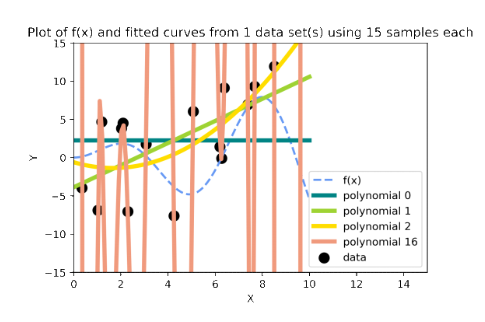
\includegraphics{1b.png}
                    \begin{center}
                        \emph{Image from page 8 of January 27th's Notes}
                    \end{center}
          \end{itemize}
    \item The relationship between the features  $\{X_1 ... X_p\}$ and the response $(Y)$ is highly non-linear.
          \begin{itemize}
              \item waffle
          \end{itemize}
    \item The variance of the noise terms, $\{X_1 ... X_p\}$, is extremely high
          \begin{itemize}
              \item When the noise of the data is extremely high, it becomes more difficult to fit a model to it as the future data may not share the variance to such a magnitude. This is because all noise is absolutely independent and irreducible, and predicting future noise is impossible. This model could be either Over or Under fitted as the approach does not set which type of behaviour is taken, regardless fitting a model to this would risk being askewed and would result in a poorer model.
          \end{itemize}
\end{enumerate}

\pagebreak
\section{Problem 2}
 [18 points total; 6 each part] You will now think of some real-life applications for machine learning. \\

\begin{enumerate}[label=(\alph*)]
    \item Describe three real-life applications in which classification might be useful. Describe the response, as well as the predictors
          \begin{itemize}
              \item Qualitative, these would be things that are attributes or properties that something could have or are )
              \item Determining the integrity of a bridge in a simulator \\\tab Predictors: Load on the bridge and materials used \\\tab Response: Stress test results if bridge broke or not
              \item
          \end{itemize}
    \item Describe three real-life applications in which regression might be useful. Describe the response, as well as the predictors.
          \begin{itemize}
              \item Quantatitive, these are often numerical values that something has
              \item Resistance of a electrical component \\\tab Predictors: Voltage, Current \\\tab Response: Voltage, Current
              \item Value of a house
              \item A person's age/height/income
          \end{itemize}
    \item Describe three real-life applications in which cluster analysis might be useful
          \begin{itemize}
              \item waffle
              \item pancake
              \item french toast
          \end{itemize}
\end{enumerate}


\pagebreak
\section{Problem 3}
We want to learn a model to predict Y, let N denote the number of samples of data. Using calculus, derive the optimal constant fucntion under mean square error
\begin{center}
    \[
        \beta_{0}^{*} = \underset{\substack{\\ \beta_{0} \epsilon \mathbb{R} } } {\text{arg min} } \frac{1}{n} \sum_{i = 1}^{n}(Y(i) - \beta_{0})^{2} \text{.}
    \]
\end{center}
make sure to check you found a minimizing $\beta_{0}$, not a maximizing $\beta_{0}$.\\



%--/Paper--

\end{document}